%%%%%%%%%%%%%%%%%%%%%%%%%%%%%%%%%%%%%%%%%%%%%%%%%%%%%%
% A Beamer template                                  %
% Based on THU beamer theme                          %
% Author: Nitesh Kumar                               %
% Date: Aug 2024                                     %
% LPPL Licensed.                                     %
%%%%%%%%%%%%%%%%%%%%%%%%%%%%%%%%%%%%%%%%%%%%%%%%%%%%%%

\documentclass[aspectratio=169]{beamer}
%\documentclass[serif]{beamer}  % for 4:3 ratio
\usepackage[T1]{fontenc} 
% \usepackage{fourier} % see "http://faq.ktug.org/wiki/uploads/MathFonts.pdf" for other options
\usepackage{hyperref}
\usepackage{latexsym,amsmath,xcolor,multicol,booktabs,calligra}
\usepackage{graphicx,pstricks,listings,stackengine}
\usepackage{lipsum}
\usepackage{tikz}

\author{Nitesh Kumar}
\title{Computational Techniques}
\subtitle{Lecture: 4}
\institute{
   nitesh.kumar@ddn.upes.ac.in \\
    School of engineering \\
    UPES, Dehradun\\
}
\date{\small \today}
\usepackage{HKUSTstyle}

% defs
\def\cmd#1{\texttt{\color{red}\footnotesize $\backslash$#1}}
\def\env#1{\texttt{\color{blue}\footnotesize #1}}
% set colors
\definecolor{hkustyellow}{RGB}{167, 131, 55}
\definecolor{hkustblue}{RGB}{1, 74, 129}
\definecolor{hkustred}{RGB}{237, 54, 118}


\lstset{
    basicstyle=\ttfamily\small,
    keywordstyle=\bfseries\color{deepblue},
    emphstyle=\ttfamily\color{deepred},    % Custom highlighting style
    stringstyle=\color{deepgreen},
    numbers=left,
    numberstyle=\small\color{halfgray},
    rulesepcolor=\color{red!20!green!20!blue!20},
    frame=shadowbox,
}

%- --- --- --- --- --- --- --- --- --- --- --- --- --- --- --- 
\begin{document}

\begin{frame}
    \titlepage
    \vspace*{-0.6cm}
    \begin{figure}[htpb]
        \begin{center}
            \includegraphics[keepaspectratio, scale=0.2]{pic/upesLogo.jpg}
        \end{center}
    \end{figure}
\end{frame}

\begin{frame}{Agenda}
\tableofcontents[sectionstyle=show,
subsectionstyle=show/shaded/hide,
subsubsectionstyle=show/shaded/hide]
\end{frame}

% Introduction --- --- --- --- --- --- --- --- --- --- --- --- 

\section{Introduction}

\begin{frame}{Course Objectives}
    \begin{enumerate}
        \item Learning fundamentals of operating system: Linux
        \item Writing computer codes using vim editor in Linux
        \item Elementary concepts of Python (Computer language)
        \item Elementary concepts of technical writing using {\LaTeX}
        \item Plotting of graphs using \texttt{Gnuplot} 
        \item Data analysis using \texttt{Gnuplot}
    \end{enumerate}
\end{frame}


% Literature Review --- --- --- --- --- --- --- --- --- --- --- 
\section{Syllabus}

\begin{frame}{Syllabus}
\begin{block}{Units}
\end{block}

\begin{enumerate}
    \item Unit 1: Introduction to Linux and Scientific Computing : 7 lecture hours
    \item Unit 2: Programming with Python : 11 lecture hours
    \item Unit 3: Scientific word processing : 6 lecture hours
    \item Unit 4: Data analysis and visualization : 6 lecture hours
\end{enumerate}
    
\end{frame}

\begin{frame}{Unit 1: Introduction to Linux and Scientific computing}
\begin{enumerate}
    \item Basics of Linux operating system 
    \item Linux commands 
    \item Vi and vim editors
    \item Computer architecture and organization 
    \item Number system and 
    \item Floating point representation 
    \item Underflow and overflow
    \item Errors in scientific computation 
\end{enumerate}

\end{frame}

\begin{frame}{Unit 2: Programming with Python}
\begin{enumerate}
    \item Introduction to Python
    \item Python literals, Operators, Variables 
    \item Loops and logic operations 
    \item Lists, functions, scopes in Python
    \item Tuples and dictionaries 
    \item Modules and packages 
    \item Errors and Exceptions 
    \item Characters and strings 
    \item Basic concepts of Object oriented programming (oop)
    \item Dealing with files 
    \item Numpy and Pandas 
\end{enumerate}
\end{frame}

\begin{frame}{Unit 3: Scientific word processing}

   \begin{enumerate}
       \item Introduction to {\LaTeX}
       \item Preparing a basic {\LaTeX} file
       \item Document classes and compiling a {\LaTeX} file
       \item Formula and equation representation
       \item Preparing figures and tables
       \item Preparing bibliography and citation 
   \end{enumerate}

\end{frame}


\begin{frame}{Unit 4: Data Analysis and visualization}

\begin{enumerate}
    \item Introduction to Gnuplot
    \item Basic Gnuplot commands 
    \item Plotting data from a file
    \item Saving and exporting data
    \item Data analysis with Gnuplot
\end{enumerate}
\end{frame}




% Unit 1 --- --- --- --- 
\section{Unit 1}
\begin{frame}{Introduction to Linux and Scientific computing}
    \begin{block}{Computer}
        -- A machine that `process' information:
    \end{block}

    \begin{enumerate}
        \item Store the data
        \item Retrieve the data
        \item Process the data
    \end{enumerate}

    \vskip1cm

    Examples: Laptop, Desktop, Servers, Mobiles, Tablets, Smart wearable, etc. 
\end{frame}

\begin{frame}{Parts of computers}

% hardware and software
\begin{block}{Hardware}
    -- Physical components of a computer \\
    e.g. CPU, Monitor, Keyboard, Mouse, etc.
\end{block}

\begin{block}{Software}
    -- Programs that run on a computer \\
    e.g. Operating system, Application software, etc.
\end{block}
    
\end{frame}


% create a frame linking software to Operating system
\begin{frame}{Operating System}
    \begin{block}{Operating System}
        -- A software that manages the hardware and software resources of a computer.
    \end{block}

    \begin{block}{Functions}
        \begin{enumerate}
            \item Memory management: RAM, ROM, Cache
            \item Processor management: CPU, Cores, Threads
            \item Device management: Input, Output, Storage
            \item File management: File system, Directories
            \item Security: User authentication, Data protection, etc.
        \end{enumerate}
    \end{block}

\end{frame}

% create a frame to list the available operating systems and their devices 
\begin{frame}{Operating Systems}
    \begin{block}{Types of Operating Systems}
        \begin{enumerate}
            \item Windows : Microsoft (PC) [Date of release: 1985]
            \item Mac OS : Apple (Mac) [Date of release: 1984]
            \item Linux : Open source (PC and Servers) [Date of release: 1991]
            \item Unix : Bell Labs (Servers) [Date of release: 1969]
            \item Android : Google (Mobiles) [Date of release: 2008]
            \item iOS : Apple (Mobiles) [Date of release: 2007]
            \item Chrome OS : Google (Chromebooks) [Date of release: 2009]
        \end{enumerate}
    \end{block}
\end{frame}

% Advantages of Linux over other operating systems
\begin{frame}{Advantages of Linux}
    \begin{block}{Advantages}
        \begin{enumerate}
            \item Free and open source: No license fee
            \item Secure: Less prone to virus attacks
            \item Stable: Less prone to crashes
            \item Customizable: Can be modified as per requirement
            \item Supports multiple users: Multiple users can work on a single system
            \item Supports multiple file systems: Ext4, NTFS, FAT32, etc.
            \item Supports multiple programming languages: C, C++, Python, Java, etc.
        \end{enumerate}
    \end{block}

\end{frame}

\begin{frame}{History of Linux Operating System}
    \begin{block}{History}
        \begin{enumerate}
            \item Developed by Linus Torvalds in 1991
            \item Based on Unix operating system
            \item Open source: Free to use and modify
            \item Supports multiple platforms: PC, Servers, Embedded systems, etc.
            \item Supports multiple file systems: Ext4, NTFS, FAT32, etc.
            \item Supports multiple programming languages: C, C++, Python, Java, etc.
        \end{enumerate}
    \end{block}
\end{frame}

% definition of distribution and examples
\begin{frame}{Linux Distribution}
    \begin{block}{Distribution}
        -- A collection of software that is based on the Linux kernel.
    \end{block}

    \begin{block}{Examples}
        \begin{enumerate}
            \item Ubuntu : Developed by Canonical Ltd.
            \item Fedora : Developed by Red Hat Inc.
            \item Debian : Developed by Debian Project
            \item CentOS : Developed by CentOS Project
            \item Arch Linux : Developed by Arch Linux Project
            \item Kali Linux : Developed by Offensive Security
        \end{enumerate}
    \end{block}
\end{frame}

% show the Linux terminal and commands
\section{Linux Terminal and Commands}
% show Linux terminal in a frame
\begin{frame}{Linux Terminal}
    \begin{block}{Terminal}
        -- A command line interface to interact with the operating system.
    \end{block}

    % show the terminal image
    \begin{figure}[htpb]
        \begin{center}
            \includegraphics[keepaspectratio, scale=0.25]{pic/linux_terminal.png}
        \end{center}
    \end{figure}
\end{frame}

% show Linux commands in a frame and allowframebreaks
\begin{frame}{Linux Commands}
    \begin{block}{Basic Syntax}

        \begin{center}
            \texttt{\$ command [options] [arguments]}
        \end{center}
        
    \end{block}


    \begin{block}{Commands}
        \begin{enumerate}
            \item \texttt{ls} : List files and directories
            \item \texttt{cd} : Change directory
            \item \texttt{pwd} : Present working directory
            \item \texttt{cp} : Copy files
            \item \texttt{mv} : Move files
            \item \texttt{rm} : Remove files
            \item \texttt{mkdir} : Make directory
        \end{enumerate}
    \end{block}

\end{frame}

%  create a slide to encourage students to try these commands in the terminal and explore more commands
\begin{frame}{Try these commands}
    \begin{block}{Exercise}
        \begin{enumerate}
            \item Open the terminal
            \item Type the command: \texttt{ls}
            \item Type the command: \texttt{pwd}
            \item Type the command: \texttt{cd} Downloads
            \item Type the command: \texttt{mkdir} MyFolder
            \item Type the command: \texttt{cp} file1 file2
            \item Type the command: \texttt{mv} file2 MyFolder/
            \item Type the command: \texttt{rm} file1
        \end{enumerate}
    \end{block}
\end{frame}

% ask students to download the Linux terminal quiz using QR code and solve it
% They can use google to find the answers
% Paste the QR on right side of the slide and ask them to scan it


% create two partition in a slide: left 60% for the content and right 40% for the image
\begin{frame}
    \begin{columns}
        \begin{column}{0.6\textwidth}
            \begin{block}{Instructions}
                \begin{enumerate}
                    \item Download the quiz using the QR code.
                    \item Solve the quiz by typing the commands in the terminal.
                    \item Use Google to find the answers if you are stuck.
                    \item Try it on your machines or use online terminals (e.g. JSLinux).
                    \item 10 Minutes time to solve the quiz.
                    % \item Submit the quiz (Just answers) by the end of next class.
                    \item Extra points for attempting Advanced questions.
                \end{enumerate}
            \end{block}
        \end{column}
        \begin{column}{0.4\textwidth}
            % show the terminal image
            \begin{figure}[htpb]
                \begin{center}
                    \includegraphics[keepaspectratio, scale=0.25]{pic/linux_quiz_qr.png}
                \end{center}
            \end{figure}
        \end{column}
    \end{columns}
\end{frame}

\section{Editors}

% create a slide on Editors in Linux and show the vim editor
\begin{frame}{Editors in Linux}
    \begin{block}{Editors}
        -- A software to write and edit text files, codes, and scripts.
    \end{block}

    \begin{block}{Types}
        \begin{enumerate}
            \item Command line editors: Vi, Vim, Nano.
            \item Graphical editors: Gedit, Kate, Emacs.
        \end{enumerate}
    \end{block}
\end{frame}

% Slide 1: History of Vi and Vim Editors
\begin{frame}{History of Vi and Vim Editors}
    \begin{itemize}
        \item \textbf{Vi Editor:} 
        \begin{itemize}
            \item Developed by Bill Joy in 1976.
            \item Part of the Berkeley Software Distribution (BSD).
            \item Originally designed for UNIX systems.
        \end{itemize}
        \item \textbf{Vim Editor:} 
        \begin{itemize}
            \item Created by Bram Moolenaar in 1991.
            \item Stands for "Vi IMproved".
            \item Aimed to add more features to the original Vi editor.
        \end{itemize}
    \end{itemize}
\end{frame}

% Slide 2: Importance of Vi and Vim Editors
\begin{frame}{Importance of Vi and Vim Editors}
    \begin{itemize}
        \item \textbf{Efficiency:} 
        \begin{itemize}
            \item Highly efficient for text editing, especially for programmers.
            \item Commands are optimized for speed and minimal keystrokes.
        \end{itemize}
        \item \textbf{Universality:} 
        \begin{itemize}
            \item Available by default on most UNIX/Linux systems.
            \item Vi is a standard editor in many environments.
        \end{itemize}
        \item \textbf{Extensibility (Vim):} 
        \begin{itemize}
            \item Vim supports plugins, scripts, and custom configurations.
            \item Highly customizable for various use cases.
        \end{itemize}
    \end{itemize}
\end{frame}



\begin{frame}{Modes of Operation in Vi and Vim Editors}
    There are Three modes of operation in Vi and Vim editors:
    \begin{block}{Modes}
        \begin{enumerate}
            \item \textbf{Command Mode:} Default mode for navigation and editing.
            \item \textbf{Insert Mode:} For inserting text into the file.
            \item \textbf{Last Line Mode:} For executing commands and saving files.
        \end{enumerate}
    \end{block}
    
\end{frame}

\begin{frame}{1. Command Mode}
    \begin{enumerate}
        \item vi starts in Command Mode.
        \item Interprets characters as commands (not displayed).
        \item Allows navigation, deletion, copying, and pasting of text.
        \item Press [Esc] to enter Command Mode from any other mode.
        \item Pressing [Esc] in Command Mode will beep or flash the screen.
    \end{enumerate}
\end{frame}


\begin{frame}{2. Insert Mode}
    \begin{enumerate}
        \item Enables insertion of text into the file.
        \item Everything typed in this mode is interpreted as input.
        \item vi always starts in Command Mode.
        \item To enter text, you must be in Insert Mode.
        \item To enter Insert Mode, type \texttt{i}.
        \item Press [Esc] to exit Insert Mode and return to Command Mode.
    \end{enumerate}    
\end{frame}

\begin{frame}{3. Last Line Mode}
    \begin{enumerate}
        \item Invoked by typing a colon [:].
        \item Cursor jumps to the last line of the screen.
        \item vi waits for a command in this mode.
        \item Enables tasks like saving files and executing commands.
        \item To save a file, type \texttt{:w} and press [Enter].
        \item To quit vi, type \texttt{:q} and press [Enter].
    \end{enumerate}
\end{frame}


\begin{frame}{Vim Editor}
    \begin{block}{Vim}
        -- A text editor based on Vi editor. 
        To open a file in vim editor:
        \\ \texttt{\$ vim my\_first\_file.txt}
    \end{block}

    % show the vim editor image
    \begin{figure}[htpb]
        \begin{center}
            \includegraphics[keepaspectratio, scale=0.25]{pic/vim_editor.png}
        \end{center}
    \end{figure}
\end{frame}



% Slide 3: Usage of Vi and Vim Editors
\begin{frame}{Usage of Vi and Vim Editors}
    \begin{itemize}
        \item \textbf{Basic Commands:} 
        \begin{itemize}
            \item \texttt{:w} - Save file
            \item \texttt{:q} - Quit editor
            \item \texttt{dd} - Delete a line
            \item \texttt{yy} - Yank (copy) a line
            \item \texttt{p} - Paste text
        \end{itemize}
        \item \textbf{Advanced Features (Vim):} 
        \begin{itemize}
            \item \texttt{:split} - Split window
            \item \texttt{:vsplit} - Vertical split
            \item \texttt{:!command} - Execute shell commands
            \item Plugin support for additional functionalities.
        \end{itemize}
    \end{itemize}
\end{frame}


% Give the class a task to open a file in vim editor and try these commands
\begin{frame}
    \begin{block}{Exercise}
        \begin{enumerate}
            \item Open a file in Vim editor: \texttt{\$ vim my\_first\_file.txt}
            \item Type some text in the file.
            \item Save the file: Press [Esc], then type \texttt{:w} and press [Enter].
            \item Quit the editor: Press [Esc], then type \texttt{:q} and press [Enter].
            \item Open the file again and try other commands.
            \item Get the Vim cheat sheet for more commands and try them.
        \end{enumerate}
    \end{block}
\end{frame}


\section[Number system]{Computer Architecture and Organization}

\begin{frame}{Computer Architecture and Organization}
    
    \begin{center}
        \resizebox{.75\textwidth}{!}{% 
        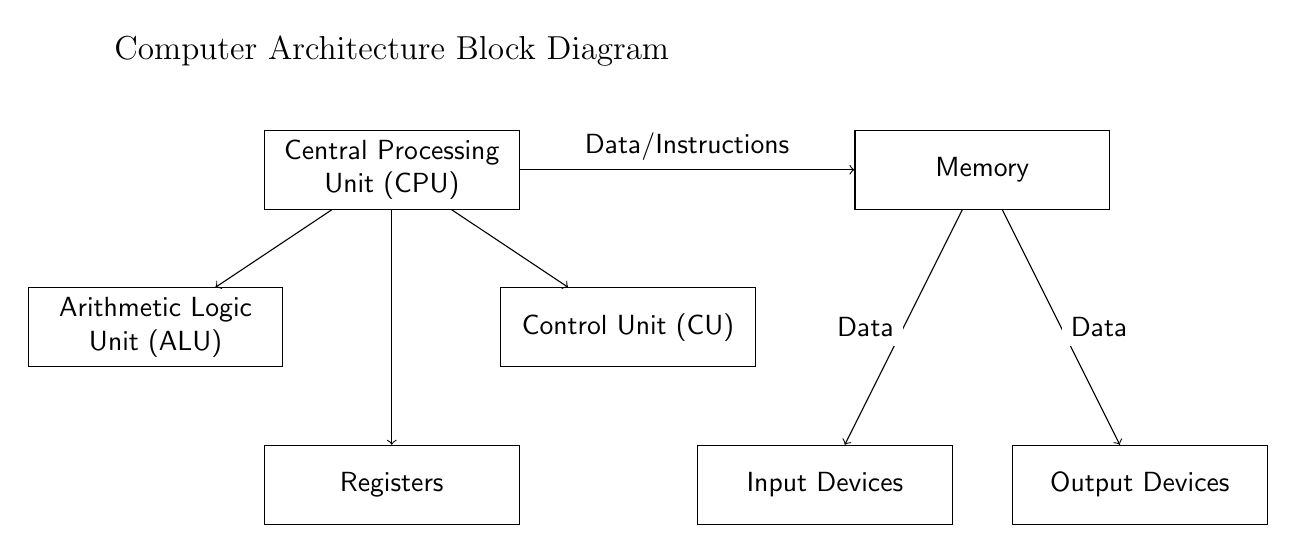
\begin{tikzpicture}[node distance=2cm, every node/.style={fill=white, font=\sffamily}, align=center]
            % Define blocks
            \node (cpu) [rectangle, draw, text width=3cm, minimum height=1cm] {Central Processing Unit (CPU)};
            \node (alu) [rectangle, draw, below of=cpu, text width=3cm, minimum height=1cm, xshift=-3cm] {Arithmetic Logic Unit (ALU)};
            \node (cu) [rectangle, draw, below of=cpu, text width=3cm, minimum height=1cm, xshift=3cm] {Control Unit (CU)};
            \node (registers) [rectangle, draw, below of=cpu, text width=3cm, minimum height=1cm, yshift=-2cm] {Registers};
            
            \node (memory) [rectangle, draw, right of=cpu, xshift=5.5cm, text width=3cm, minimum height=1cm] {Memory};
            
            \node (input) [rectangle, draw, below of=memory, xshift=-2cm, yshift=-2cm, text width=3cm, minimum height=1cm] {Input Devices};
            \node (output) [rectangle, draw, below of=memory, xshift=2cm, yshift=-2cm, text width=3cm, minimum height=1cm] {Output Devices};
            
            % Draw arrows
            \draw[->] (cpu) -- (alu);
            \draw[->] (cpu) -- (cu);
            \draw[->] (cpu) -- (registers);
            
            \draw[->] (cpu) -- (memory) node[midway, above] {Data/Instructions};
            \draw[->] (memory) -- (input) node[midway, left] {Data};
            \draw[->] (memory) -- (output) node[midway, right] {Data};
            
            % Labels
            \node [above of=cpu, yshift=-0.5cm, font=\large] {Computer Architecture Block Diagram};
        \end{tikzpicture}
        }
        \end{center}
\end{frame}


% create a slide on how the computers stores the information
\begin{frame}{How Computers Store Information}
    \begin{itemize}
        \item \textbf{Binary System:}
        \begin{itemize}
            \item Computers use the binary number system (0s and 1s) to represent all types of data.
            \item A bit (binary digit) is the smallest unit of data in a computer.
            \item 8 bits form a byte, which can represent 256 different values.
        \end{itemize}
        
        \item \textbf{Memory Hierarchy:}
        \begin{itemize}
            \item \textbf{Registers:} Small, fast storage areas in the CPU used for temporary data.
            \item \textbf{Cache:} Intermediate storage between registers and main memory, faster than RAM.
            \item \textbf{Main Memory (RAM):} Stores data and instructions that the CPU needs in real-time.
            \item \textbf{Secondary Storage:} Non-volatile storage like hard drives, SSDs, where data is stored long-term.
        \end{itemize}
        
        \item \textbf{Data Representation:}
        \begin{itemize}
            \item \textbf{Characters:} Stored using encoding schemes like ASCII or Unicode.
            \item \textbf{Numbers:} Stored as integers or floating-point representations.
            \item \textbf{Images and Sound:} Stored as a series of bits representing pixel values or sound waveforms.
        \end{itemize}
        
        \item \textbf{File Systems:}
        \begin{itemize}
            \item Organizes and manages how data is stored and retrieved on secondary storage devices.
        \end{itemize}
    \end{itemize}
\end{frame}


% Slide 1: Introduction to Number Systems in Computing
\begin{frame}{Introduction to Number Systems in Computing}
    \begin{itemize}
        \item \textbf{Number Systems:} 
        \item \textbf{Binary System:} 
        \begin{itemize}
            \item Base-2 number system.
            \item Uses digits 0 and 1.
            \item Essential for representing data in digital computers.
        \end{itemize}
        \item \textbf{Other Systems:}
        \begin{itemize}
            \item \textbf{Decimal (Base-10):} Commonly used by humans.
            \item \textbf{Hexadecimal (Base-16):} Often used in programming and debugging.
            \item \textbf{Octal (Base-8):} Sometimes used in computing as a shorthand for binary.
        \end{itemize}
    \end{itemize}
\end{frame}

% Slide 2: Binary Number System
\begin{frame}{Binary Number System}
    \begin{itemize}
        \item \textbf{Base-2 System:} Each bit represents a power of 2.
        \item \textbf{Binary Digits (Bits):} 
        \begin{itemize}
            \item 0 and 1.
            \item Example: \( 1011_2 = 1 \times 2^3 + 0 \times 2^2 + 1 \times 2^1 + 1 \times 2^0 = 11_{10} \).
        \end{itemize}
        \item \textbf{Significance:} 
        \begin{itemize}
            \item Basis for all modern digital systems.
            \item Used in memory storage, data processing, and communication.
        \end{itemize}
    \end{itemize}
\end{frame}

% Slide 3: Hexadecimal and Octal Number Systems
\begin{frame}{Hexadecimal and Octal Number Systems}
    \begin{itemize}
        \item \textbf{Hexadecimal (Base-16):} 
        \begin{itemize}
            \item Digits: 0-9 and A-F (where A=10, B=11, ..., F=15).
            \item Example: \( A3_{16} = 10 \times 16^1 + 3 \times 16^0 = 163_{10} \).
            \item Used to represent large binary numbers succinctly.
        \end{itemize}
        \item \textbf{Octal (Base-8):} 
        \begin{itemize}
            \item Digits: 0-7.
            \item Example: \( 57_8 = 5 \times 8^1 + 7 \times 8^0 = 47_{10} \).
            \item Often used in digital systems as a shorthand for binary.
        \end{itemize}
    \end{itemize}
\end{frame}

% Slide 4: Conversion Between Number Systems
\begin{frame}{Conversion Between Number Systems}
    \begin{itemize}
        \item \textbf{Binary to Decimal:} 
        \begin{itemize}
            \item Example: \( 1101_2 = 1 \times 2^3 + 1 \times 2^2 + 0 \times 2^1 + 1 \times 2^0 = 13_{10} \).
        \end{itemize}
        \item \textbf{Decimal to Binary:} 
        \begin{itemize}
            \item Example: \( 13_{10} = 1101_2 \) (Divide by 2 and track remainders).
        \end{itemize}
        \item \textbf{Hexadecimal to Binary:} 
        \begin{itemize}
            \item Example: \( A3_{16} = 1010_2 0011_2 \).
        \end{itemize}
        \item \textbf{Octal to Binary:} 
        \begin{itemize}
            \item Example: \( 57_8 = 101_2 111_2 \).
        \end{itemize}
    \end{itemize}
\end{frame}

% Slide 5: Importance of Number Systems in Computer Architecture
\begin{frame}{Importance of Number Systems in Computer Architecture}
    \begin{itemize}
        \item \textbf{Data Representation:} 
        \begin{itemize}
            \item Numbers, characters, and instructions are represented in binary.
        \end{itemize}
        \item \textbf{Memory Addressing:} 
        \begin{itemize}
            \item Memory locations are often referred to using hexadecimal numbers.
        \end{itemize}
        \item \textbf{Instruction Sets:} 
        \begin{itemize}
            \item Instructions are encoded in binary to be processed by the CPU.
        \end{itemize}
        \item \textbf{Efficient Computation:} 
        \begin{itemize}
            \item Binary arithmetic is faster and simpler to implement in hardware.
        \end{itemize}
    \end{itemize}
\end{frame}

% Slide 1: Introduction to Floating-Point Representation
\begin{frame}{Introduction to Floating-Point Representation}
    \begin{itemize}
        \item \textbf{Floating-Point Numbers:} Used to represent real numbers in a form that can support a wide range of values.
        \item \textbf{Components:}
        \begin{itemize}
            \item \textbf{Sign (S):} Indicates positive or negative number.
            \item \textbf{Exponent (E):} Determines the scale (magnitude) of the number.
            \item \textbf{Mantissa (M) or Significand:} Represents the precision of the number.
        \end{itemize}
        \item \textbf{IEEE 754 Standard:}
        \begin{itemize}
            \item Commonly used format for floating-point representation.
            \item Single precision (32-bit) and double precision (64-bit) formats.
        \end{itemize}
    \end{itemize}
\end{frame}

% Slide 2: Example of Floating-Point Representation
\begin{frame}{Example of Floating-Point Representation}
    \begin{itemize}
        \item \textbf{Example:} Representing the decimal number \( -6.25 \) in IEEE 754 single precision.
        \item \textbf{Step 1: Convert to Binary}
        \begin{itemize}
            \item \( 6.25_{10} = 110.01_2 \).
            \item Sign bit \( S = 1 \) (negative number).
        \end{itemize}
        \item \textbf{Step 2: Normalize the Binary Number}
        \begin{itemize}
            \item \( 110.01_2 = 1.1001_2 \times 2^2 \).
        \end{itemize}
        \item \textbf{Step 3: Determine Exponent}
        \begin{itemize}
            \item Exponent \( E = 127 + 2 = 129 \) (in bias-127 form).
            \item Binary of 129 = \( 10000001_2 \).
        \end{itemize}
        \item \textbf{Step 4: Form the Mantissa}
        \begin{itemize}
            \item Mantissa = \( 10010000000000000000000_2 \) (23 bits).
        \end{itemize}
        \item \textbf{Final IEEE 754 Representation:}
        \begin{itemize}
            \item \( 1\;10000001\;10010000000000000000000_2 \).
            \item In hexadecimal: \( C1C80000_{16} \).
        \end{itemize}
    \end{itemize}
\end{frame}


\begin{frame}{Example of Floating-Point Representation (Double Precision)}
    \begin{itemize}
        \item \textbf{Example:} Representing the decimal number \( -6.25 \) in IEEE 754 double precision.
        \item \textbf{Step 1: Convert to Binary}
        \begin{itemize}
            \item \( 6.25_{10} = 110.01_2 \).
            \item Sign bit \( S = 1 \) (negative number).
        \end{itemize}
        \item \textbf{Step 2: Normalize the Binary Number}
        \begin{itemize}
            \item \( 110.01_2 = 1.1001_2 \times 2^2 \).
        \end{itemize}
        \item \textbf{Step 3: Determine Exponent}
        \begin{itemize}
            \item Exponent \( E = 1023 + 2 = 1025 \) (in bias-1023 form).
            \item Binary of 1025 = \( 10000000001_2 \).
        \end{itemize}
        \item \textbf{Step 4: Form the Mantissa}
        \begin{itemize}
            \item Mantissa = \( 1001000000000000000000000000000000000000000000000000_2 \) (52 bits).
        \end{itemize}
        \item \textbf{Final IEEE 754 Representation:}
        \begin{itemize}
            \item \( 1\;10000000001\;1001000000000000000000000000000000000000000000000000_2 \).
            % \item In hexadecimal: \( C01C800000000000_{16} \).
        \end{itemize}
    \end{itemize}
\end{frame}


\begin{frame}[allowframebreaks]{IEEE 754 Single Precision: Maximum, Minimum, and Special Cases}
    \begin{itemize}
        \item \textbf{IEEE 754 Single Precision Format:}
        \begin{itemize}
            \item 1 bit for sign (\(S\))
            \item 8 bits for exponent (\(E\)) with bias 127
            \item 23 bits for mantissa (\(M\)) + implicit leading 1
        \end{itemize}
        
        \framebreak
        
        \item \textbf{Maximum Number:}
        \begin{itemize}
            \item Exponent: \( E = 254 \) 
            \item Actual exponent: \( 254 - 127 = 127 \)
            \item Largest mantissa: \( M = 1 + (1 - 2^{-23}) \)
            \item Maximum value:
            \[
            (1.99999988) \times 2^{127} \approx 3.4028235 \times 10^{38}
            \]
            \item Hex representation: \( 7F7FFFFF_{16} \)
        \end{itemize}

        \framebreak
        
        \item \textbf{Minimum Normalized Positive Number:}
        \begin{itemize}
            \item Exponent: \( E = 1 \)
            \item Actual exponent: \( 1 - 127 = -126 \)
            \item Smallest normalized value:
            \[
            1.0 \times 2^{-126} \approx 1.17549435 \times 10^{-38}
            \]
            \item Hex representation: \( 00800000_{16} \)
        \end{itemize}

        \framebreak

        % \item \textbf{Smallest Subnormal Positive Number:}
        % \begin{itemize}
        %     \item Exponent: \( E = 0 \) 
        %     \item Subnormal value:
        %     \[
        %     0.0000001_2 \times 2^{-126} \approx 1.4 \times 10^{-45}
        %     \]
        %     \item Hex representation: \( 00000001_{16} \)
        % \end{itemize}

        \item \textbf{Smallest negative number:}
        \begin{itemize}
            \item Exponent: \( E = 0 \) 
            \item Mantissa: \( M = 0 \)
            \item Smallest negative value:
            \[
            -0.0 \times 2^{-126} \approx -1.17549435 \times 10^{-38}
            \]
            \item Hex representation: \( 80800000_{16} \)
        \end{itemize}

        \framebreak

        \item \textbf{Special Values:}
        % \begin{itemize}
        %     \item \textbf{Zero:}
        %     \begin{itemize}
        %         \item Positive zero: \( 00000000_{16} \)
        %         \item Negative zero: \( 80000000_{16} \)
        %     \end{itemize}
        %     \item \textbf{Infinity:}
        %     \begin{itemize}
        %         \item Positive infinity: \( 7F800000_{16} \)
        %         \item Negative infinity: \( FF800000_{16} \)
        %     \end{itemize}
        %     \item \textbf{NaN (Not a Number):}
        %     \begin{itemize}
        %         \item Exponent = 255 and mantissa \neq 0
        %         \item Example: \( 7FC00000_{16} \) (quiet NaN)
        %     \end{itemize}
        % \end{itemize}


        \begin{itemize}
            \item \textbf{Zero:}
            \begin{itemize}
                \item \textbf{Positive Zero:} 
                \[
                00000000000000000000000000000000_2
                \]
                \item \textbf{Negative Zero:} 
                \[
                10000000000000000000000000000000_2
                \]
            \end{itemize}
                
            \item \textbf{Infinity:}
            \begin{itemize}
                \item \textbf{Positive Infinity:} 
                \[
                01111111100000000000000000000000_2
                \]
                \item \textbf{Negative Infinity:} 
                \[
                11111111100000000000000000000000_2
                \]
            \end{itemize}

            \framebreak

            
            \item \textbf{NaN (Not a Number):}
            \begin{itemize}
                \item Exponent = 255 (all 1's) and mantissa \(\neq 0\)
                \item \textbf{Example:} 
                \[
                01111111110000000000000000000000_2 \text{ (quiet NaN)}
                \]
            \end{itemize}
        \end{itemize}
    \end{itemize}
\end{frame}



\begin{frame}[allowframebreaks]{Overflow, Underflow, and Precision in IEEE 754 Single Precision}
    \begin{itemize}
        \item \textbf{Overflow:}
        \begin{itemize}
            \item Occurs when a calculation produces a number larger than the maximum representable value.
            \item Example: 
            \[
            \text{Max representable} = (1.99999988) \times 2^{127}
            \]
            \item If you try to represent \( 2^{128} \) or higher, it exceeds the maximum value and results in infinity:
            \[
            2^{128} \text{ is represented as } \infty
            \]
        \end{itemize}
        
        \framebreak

        \item \textbf{Underflow:}
        \begin{itemize}
            \item Occurs when a calculation produces a number smaller than the smallest normalized positive value.
            \item Example: 
            \[
            \text{Smallest normalized value} = 1.17549435 \times 10^{-38}
            \]
            \item If you try to represent a number smaller than \( 1.4 \times 10^{-45} \), it becomes a subnormal number or zero:
            \[
            1.4 \times 10^{-45} \text{ is the smallest subnormal positive number}
            \]
        \end{itemize}

        \framebreak

        \item \textbf{Precision:}
        \begin{itemize}
            \item Precision refers to the number of significant bits used to represent a number.
            \item In single precision, 23 bits are used for the mantissa, providing about 7 decimal digits of precision.
            \item Example:
            \[
            \text{Number } 0.1_{10} \text{ in binary } = 0.00011001100110011001101_2
            \]
            \item The closest representable value in single precision may be slightly different from the exact decimal representation.
        \end{itemize}
    \end{itemize}
\end{frame}





% --- Thank you slide ---
\begin{frame}
\begin{center}
{ Thank you for listening !}
\vspace{1cm}

Nitesh Kumar \\[1em]
nitesh.kumar@ddn.upes.ac.in
\end{center}
\end{frame}

\end{document}

% create notes based on the above slides to present in the class


% Introduction
% 1. Introduction to the course
% 2. Objectives of the course
% 3. Syllabus of the course
% 4. Introduction to Linux and Scientific computing
% 5. Parts of computers
% 6. Operating System
% 7. Types of Operating Systems
% 8. Advantages of Linux
% 9. History of Linux Operating System
% 10. Linux Distribution
% 11. Linux Terminal
% 12. Linux Commands
% 13. Thank you slide
